% SI - Figure 1 Schematic
\begin{figure}[htb]
\centering
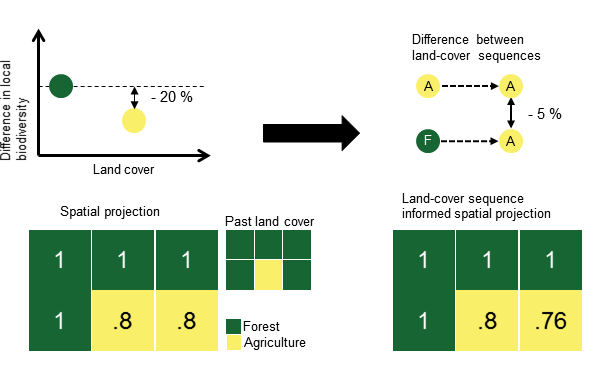
\includegraphics[width=.9\textwidth]{chapter4/SI01}
\caption{ Schematic on how spatial projections of a difference in biodiversity can be informed by models of past land-cover sequences. (\textbf{a}) First a “baseline” spatial projection is created based on the difference in local biodiversity measures between forest and agricultural sites (-20\% in local biodiversity). Knowing that past land cover in the bottom-right cell was forest covered, this baseline spatial projection is then (\textbf{b}) updated based on the specific coefficient (-5\%) from the models (Figure \ref{F04_03}) for each land-cover sequence. }
\label{SI04_01}
\end{figure}

% SI - Figure 2 Sites per change category
\begin{figure}[htb]
\centering
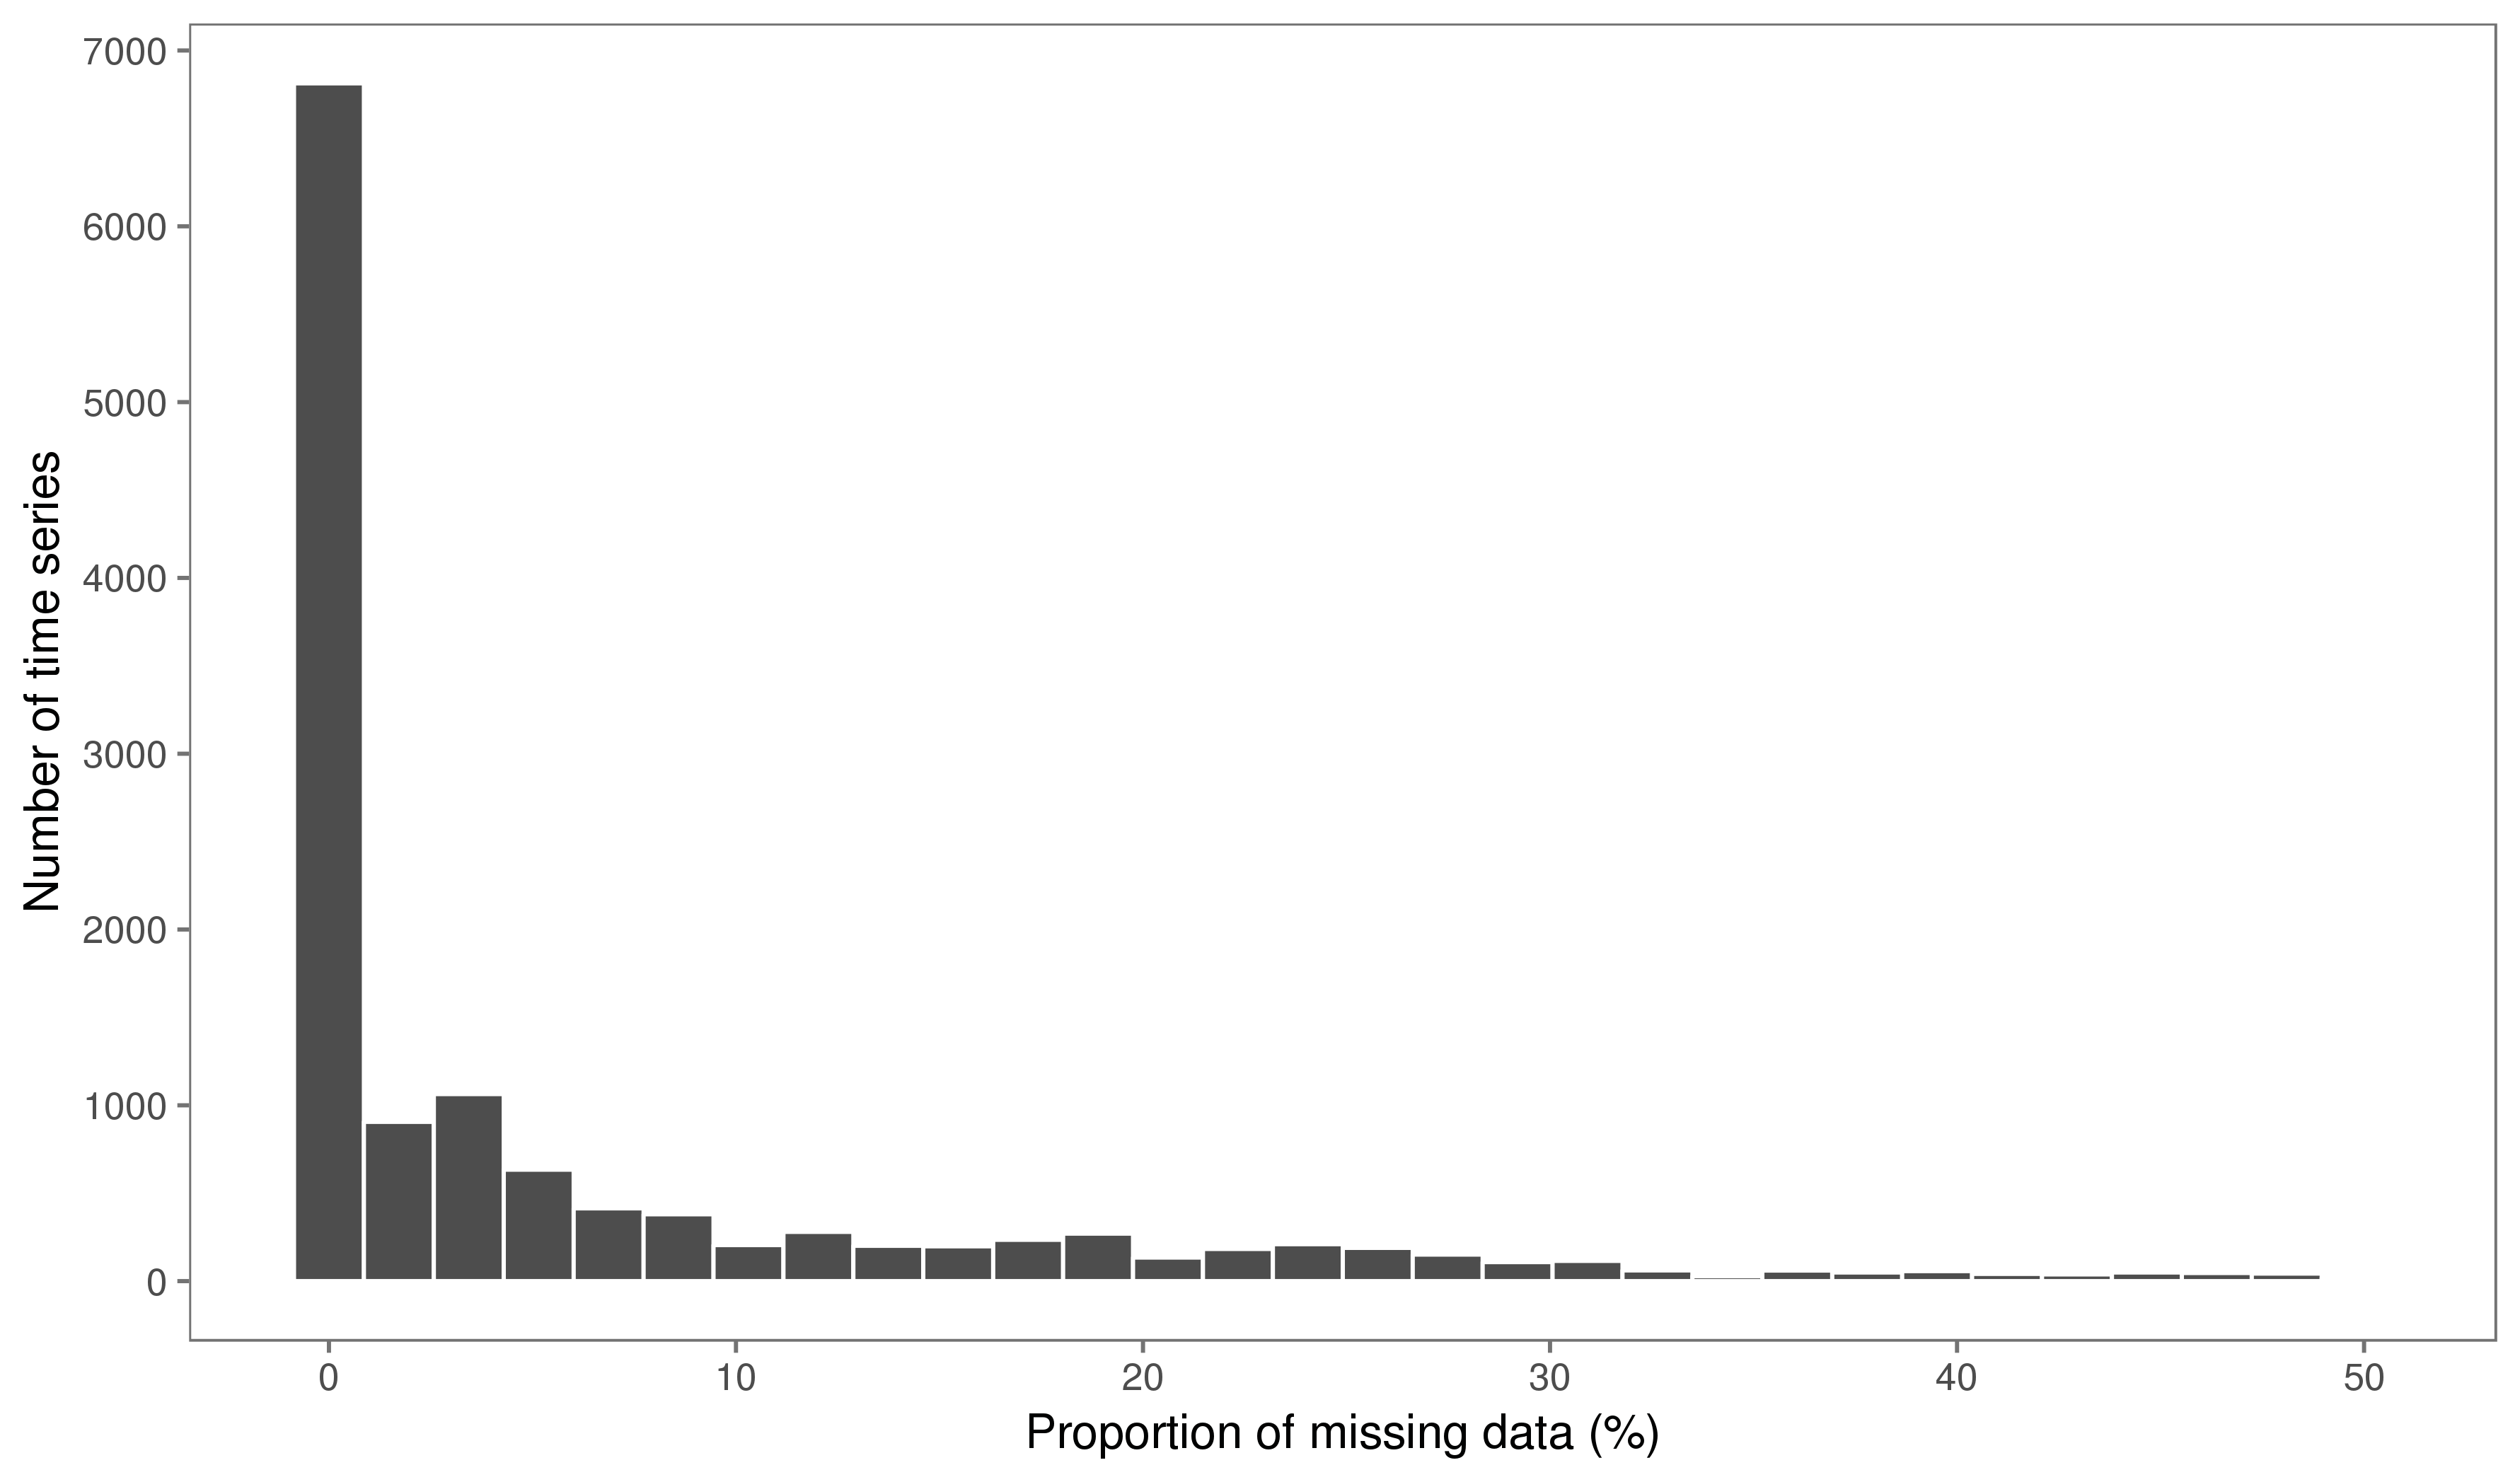
\includegraphics[width=.9\textwidth]{chapter4/SI02}
\caption{ Total number of sites (log10 transformed) without ($0$) and with ($1$) a past land-cover change. Colours indicate the land-cover category at the time of biodiversity sampling. }
\label{SI04_02}
\end{figure}

% SI - Figure 3 Main difference
\begin{figure}[htb]
\centering
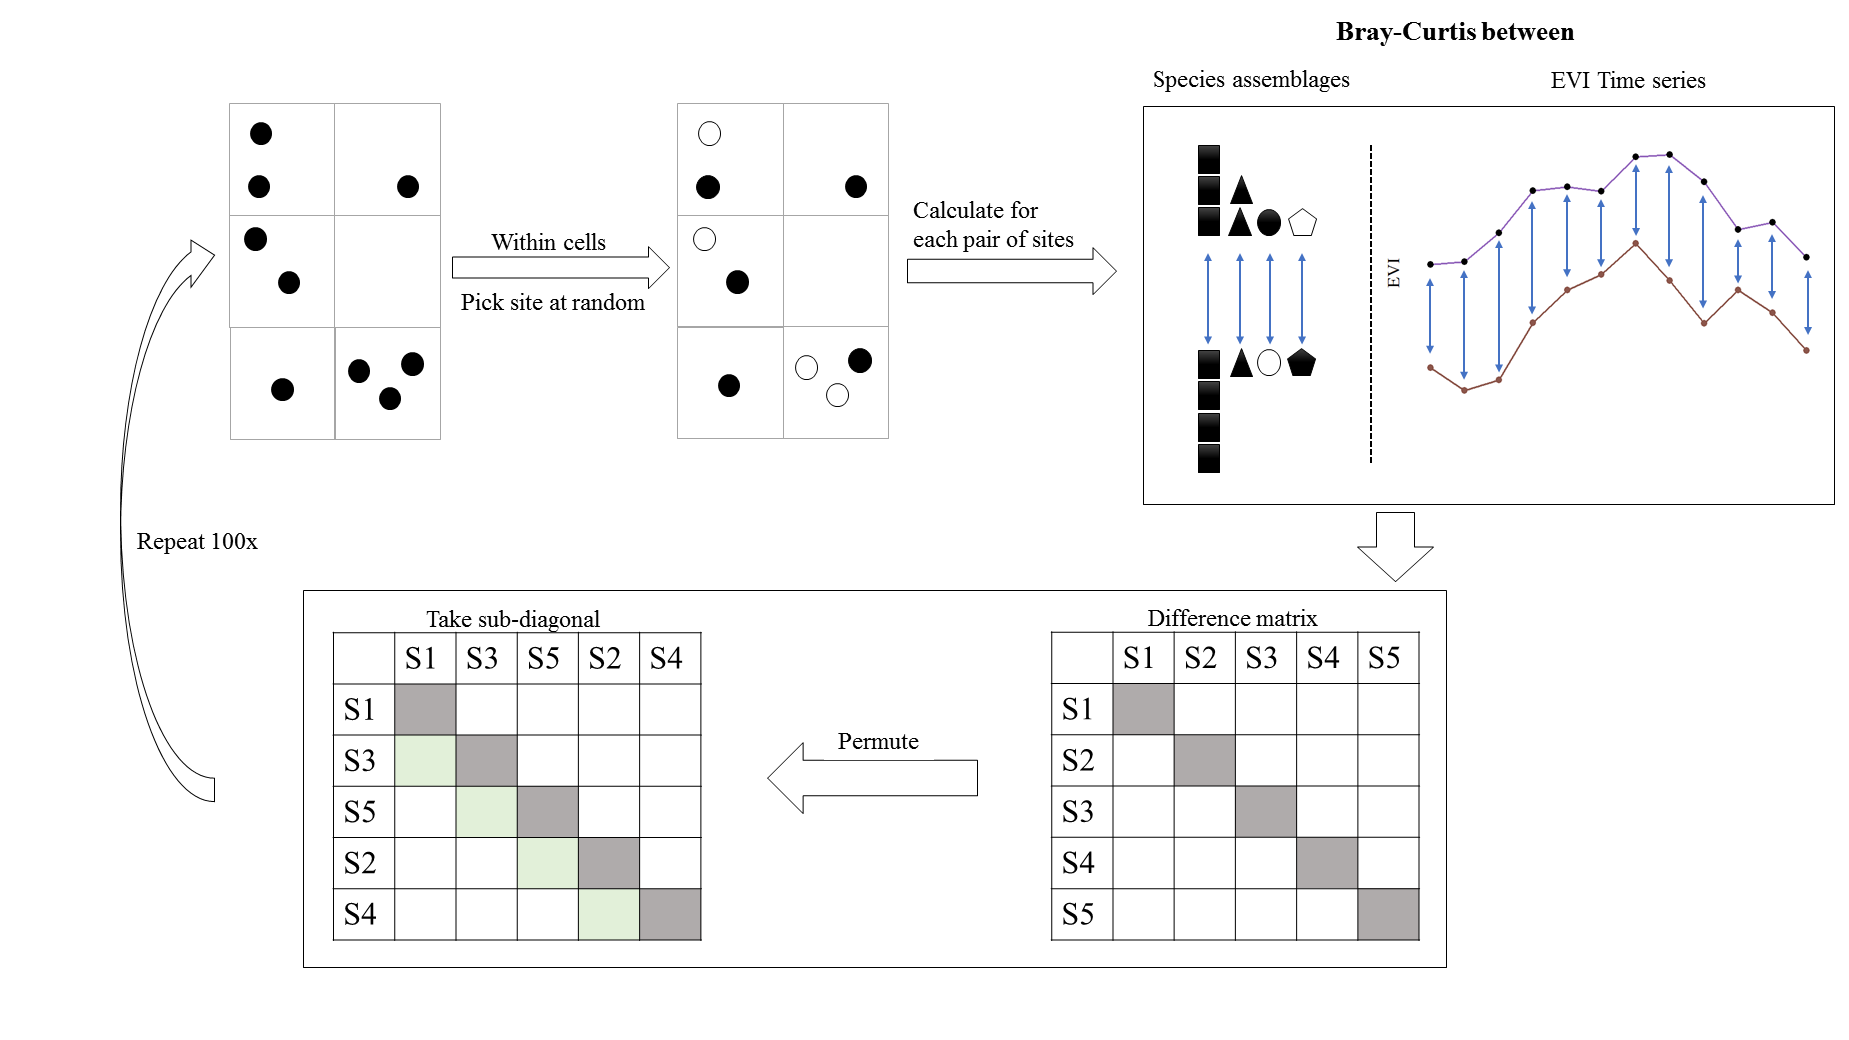
\includegraphics[width=.9\textwidth]{chapter4/SI03}
\caption{ (\textbf{a}) Globally projected difference in species richness (\%) \textendash\ weighted by vertebrate richness, see methods \textendash\ relative to local species richness in forests with zero human population density. (\textbf{b}) The predicted (unweighted) uncertainty in local species richness shown as mean absolute error (MAE). }
\label{SI04_03}
\end{figure}

% SI - Figure 4 Population difference
\begin{figure}[htb]
\centering
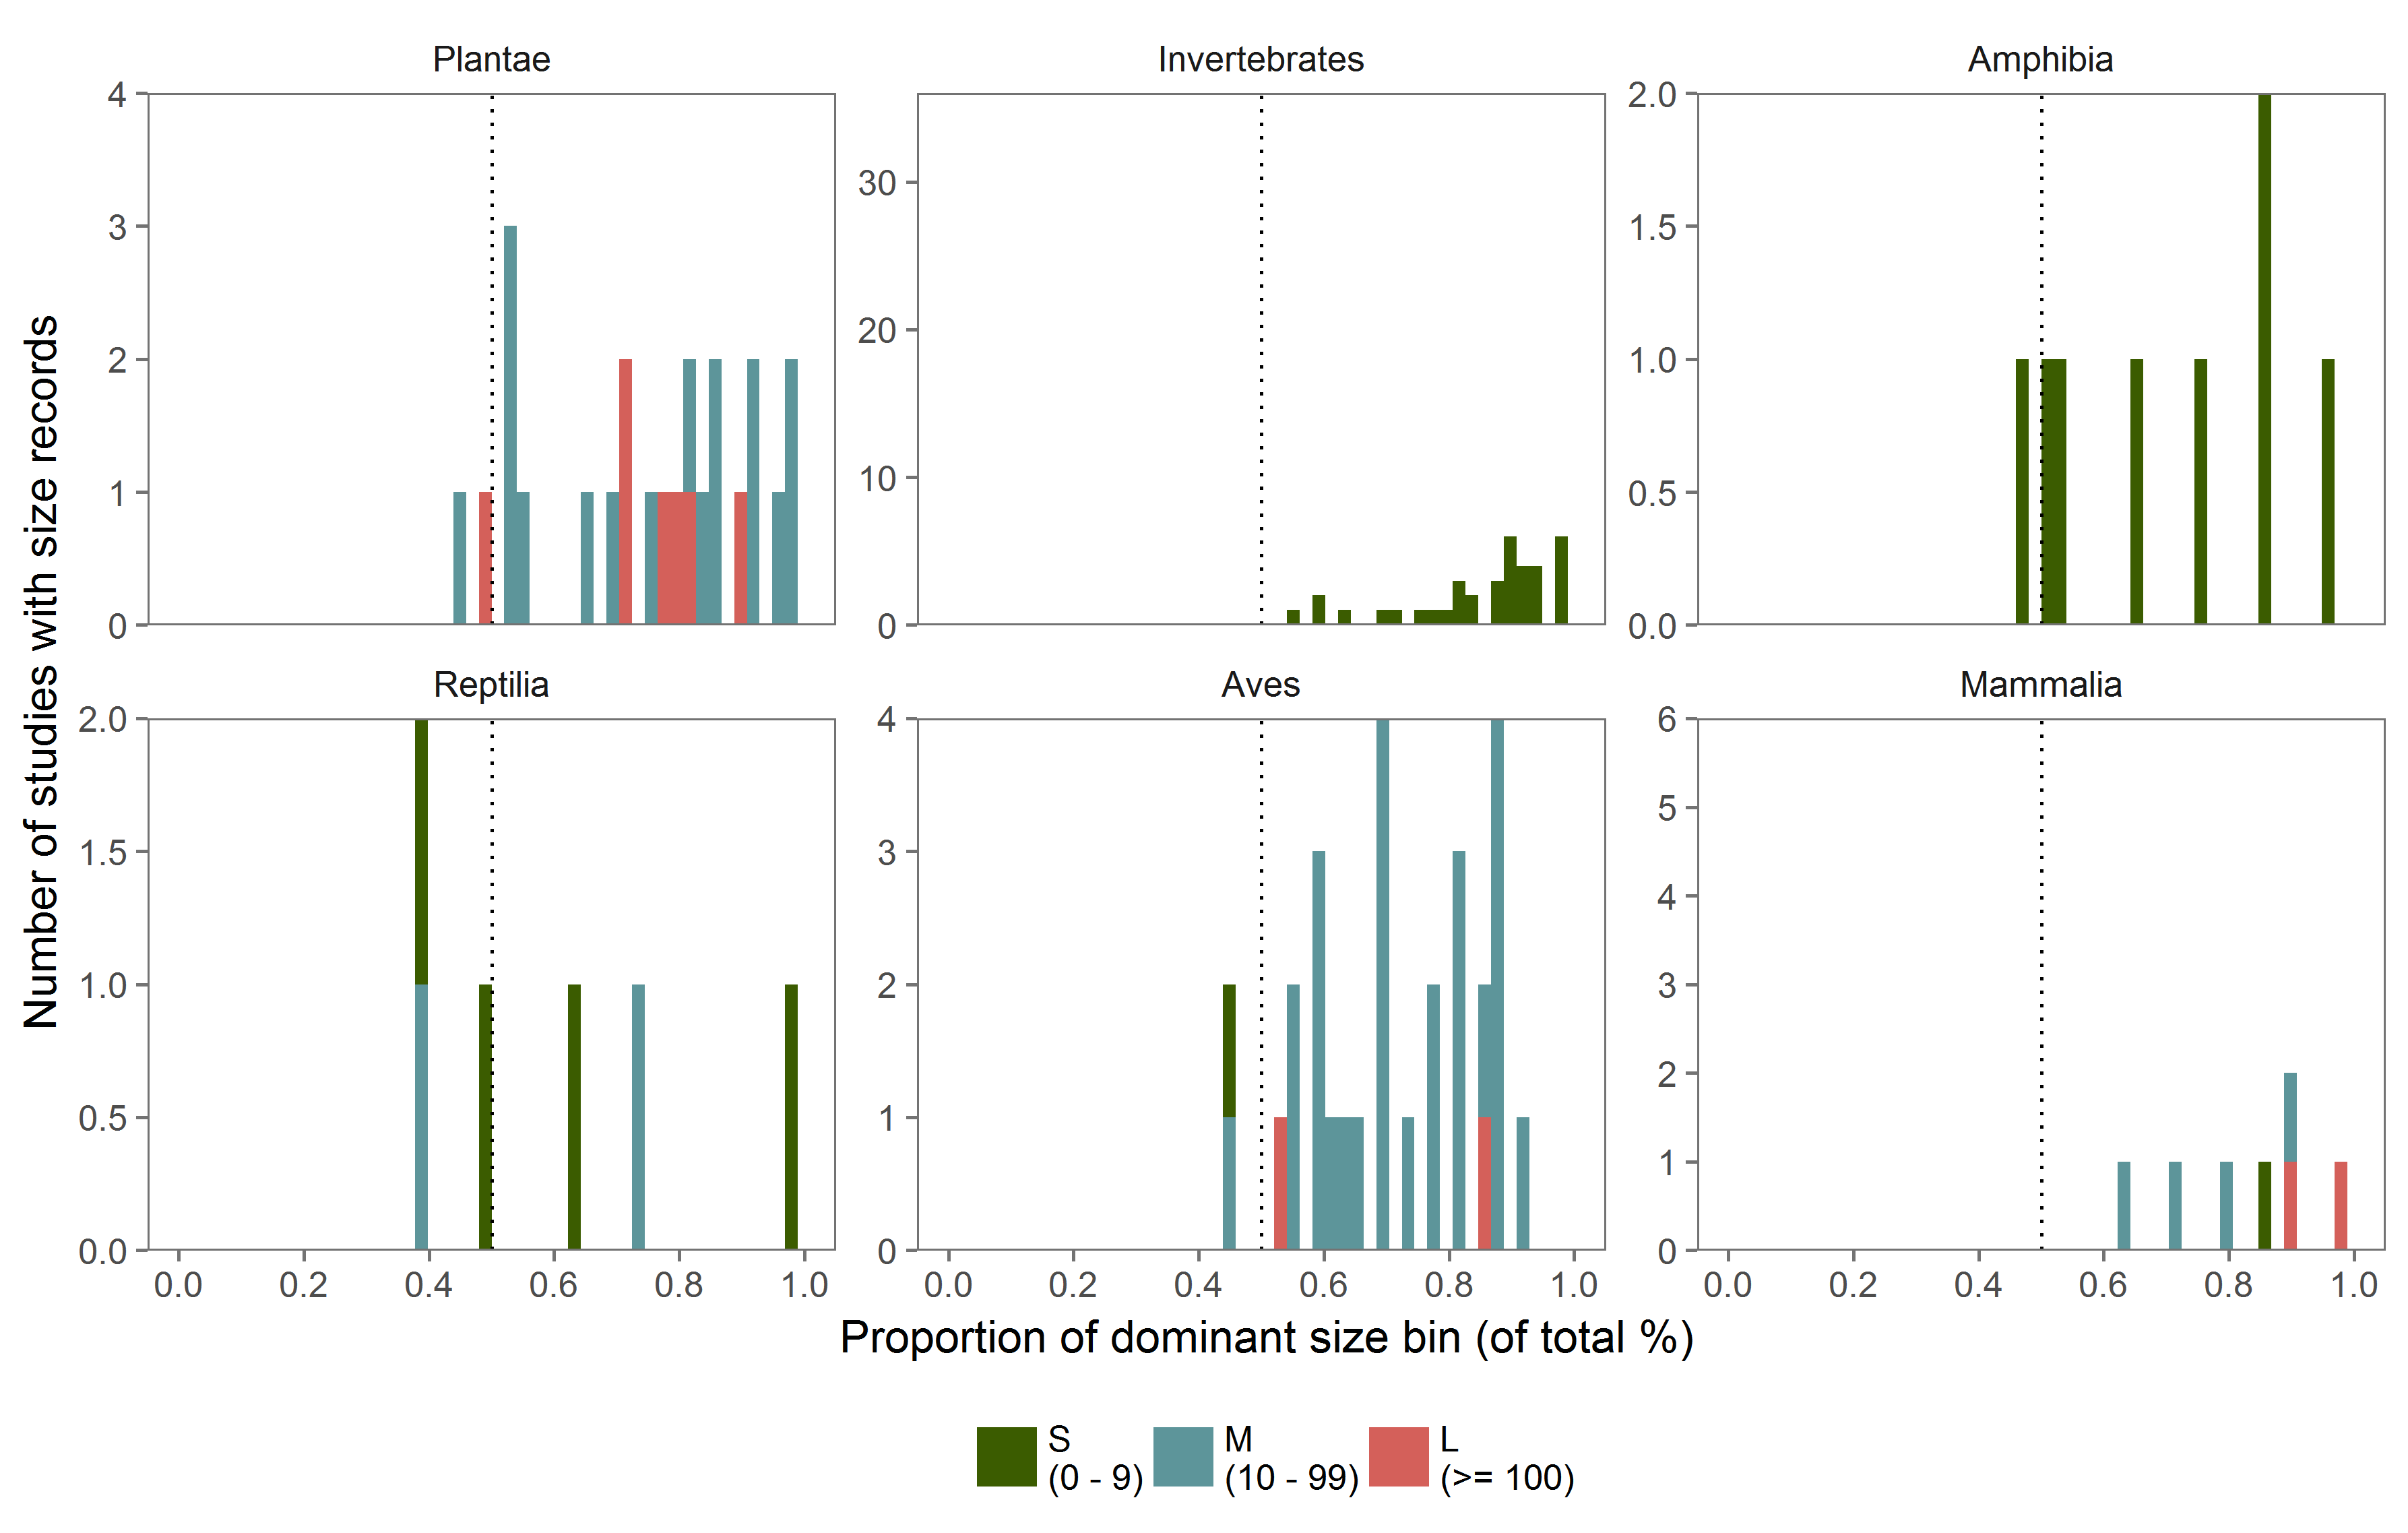
\includegraphics[width=.9\textwidth]{chapter4/SI04}
\caption{ (\textbf{a}) Difference in the effect size (linear slope) of human population density on species richness (SR), total abundance (LA) and assemblage evenness (PIE). All effects shown relative to the effect of forest cover on local biodiversity, with values greater than $0$ indicating a linear increase of the response. Error bars show the estimated standard error. (\textbf{b}) Number of PREDICTS sites per land-cover category and human population density (log\textunderscript{10}-transformed) from the global human settlement product \citep{Pesaresi2016}. }
\label{SI04_04}
\end{figure}

% SI - Figure 5 Boxplot
\begin{figure}[htb]
\centering
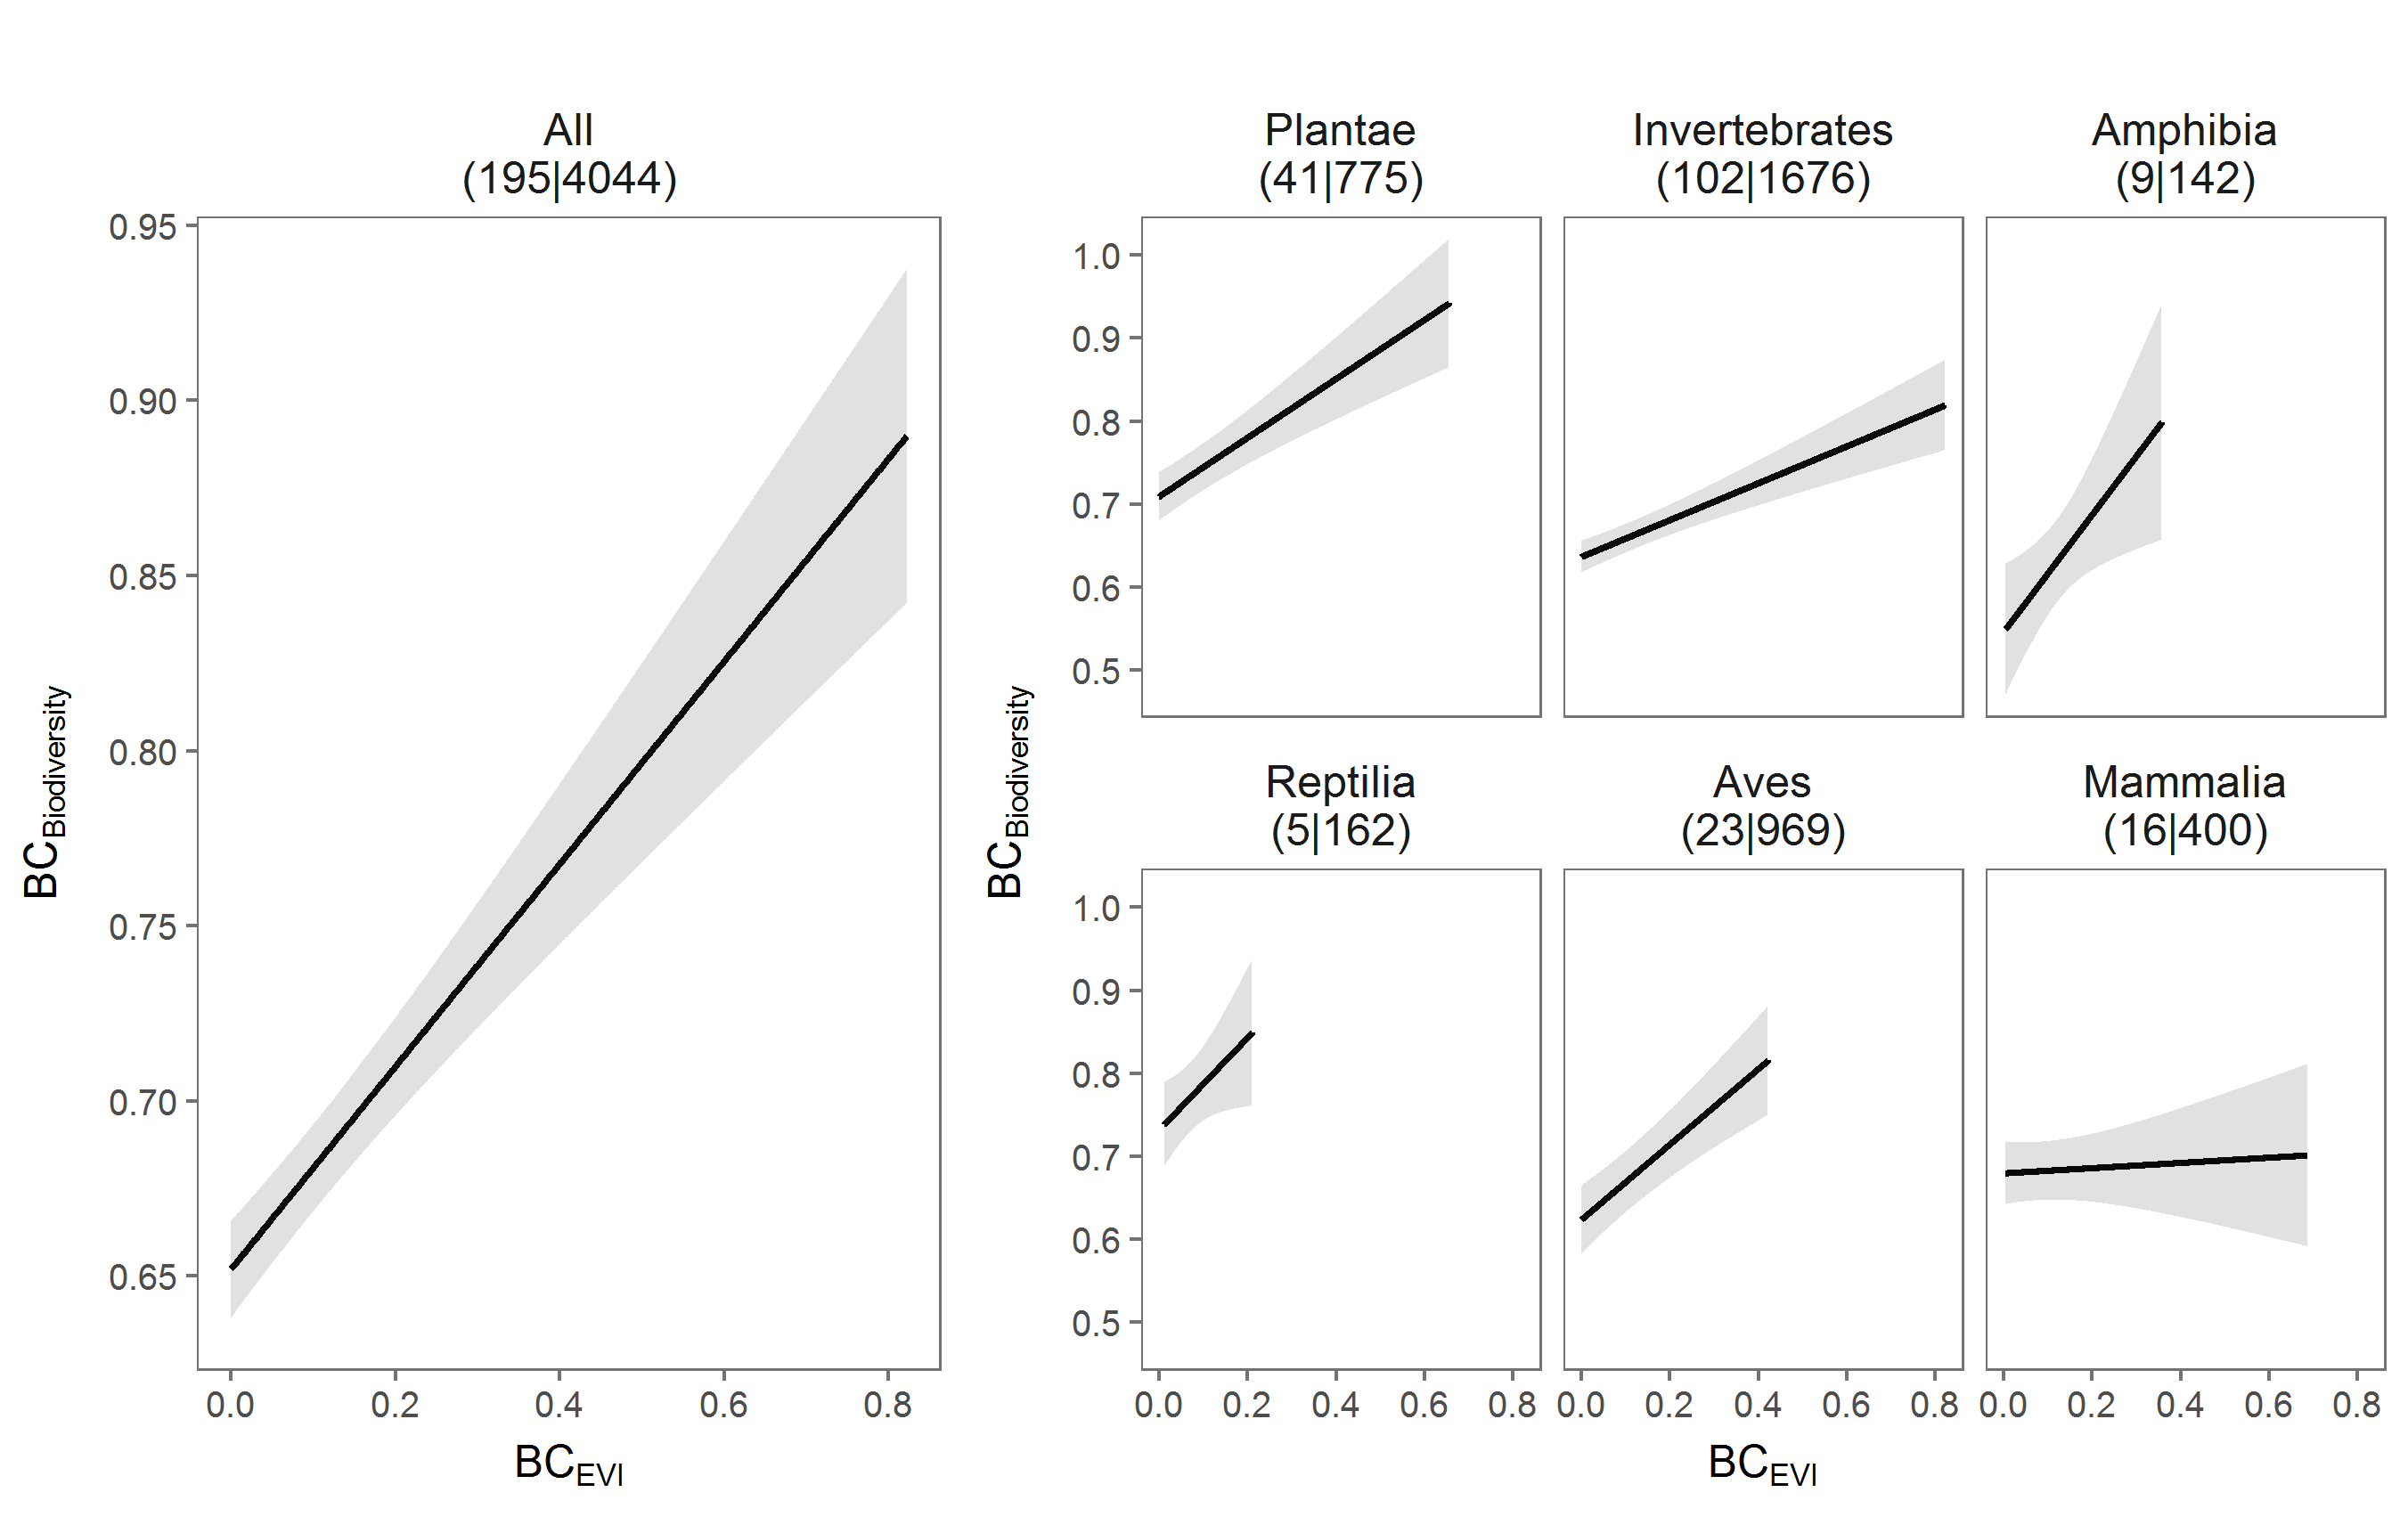
\includegraphics[width=.9\textwidth]{chapter4/SI05}
\caption{ Shows the proportion of land (in \%) with a past land-cover change in the period 2000 to 2015 relative to the total land area. Size of the points is scaled with land area (small to large). Colours indicate whether a country (data from \href{data.un.org}{data.un.org}) is considered to have high (black), middle (orange) or low (blue) income.}
\label{SI04_05}
\end{figure}

% SI - Figure 6 National abundance estimates
\begin{figure}[htb]
\centering
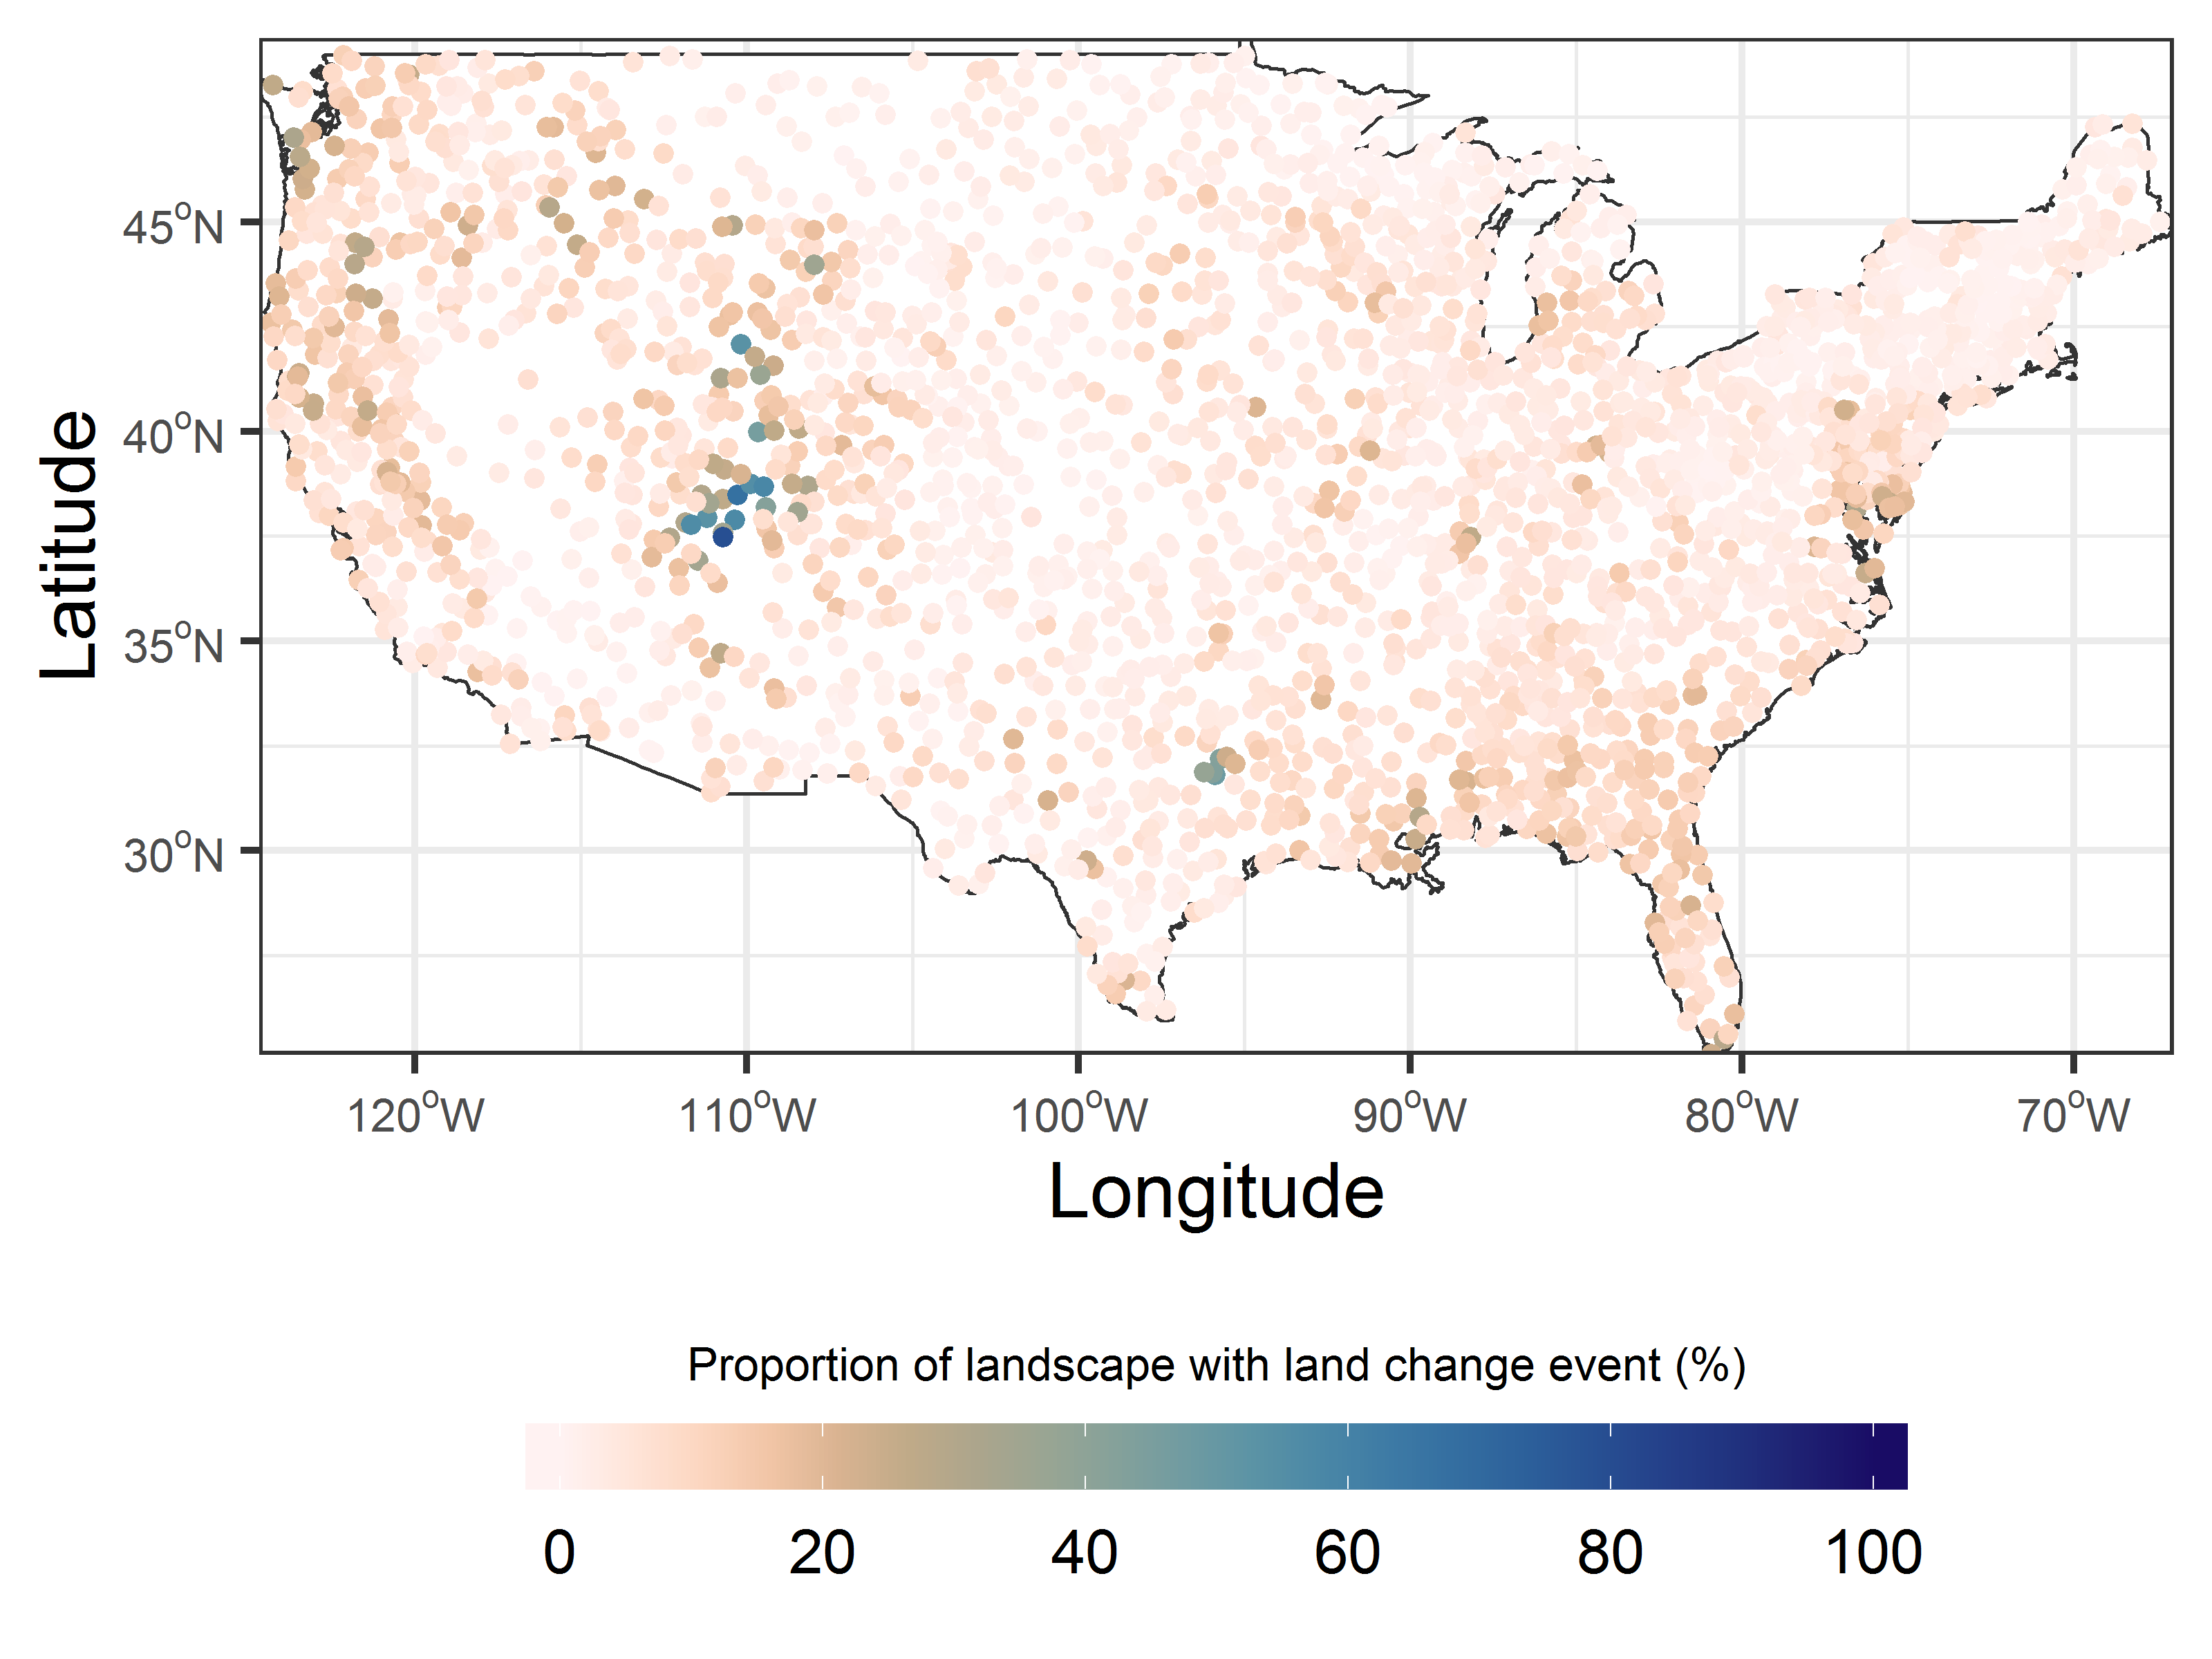
\includegraphics[width=1\textwidth]{chapter4/SI06}
\caption{ As in Figure \ref{F04_05} but for total abundance (LA). }
\label{SI04_06}
\end{figure}

% SI - Figure 7 National PIE estimates
\begin{figure}[htb]
\centering
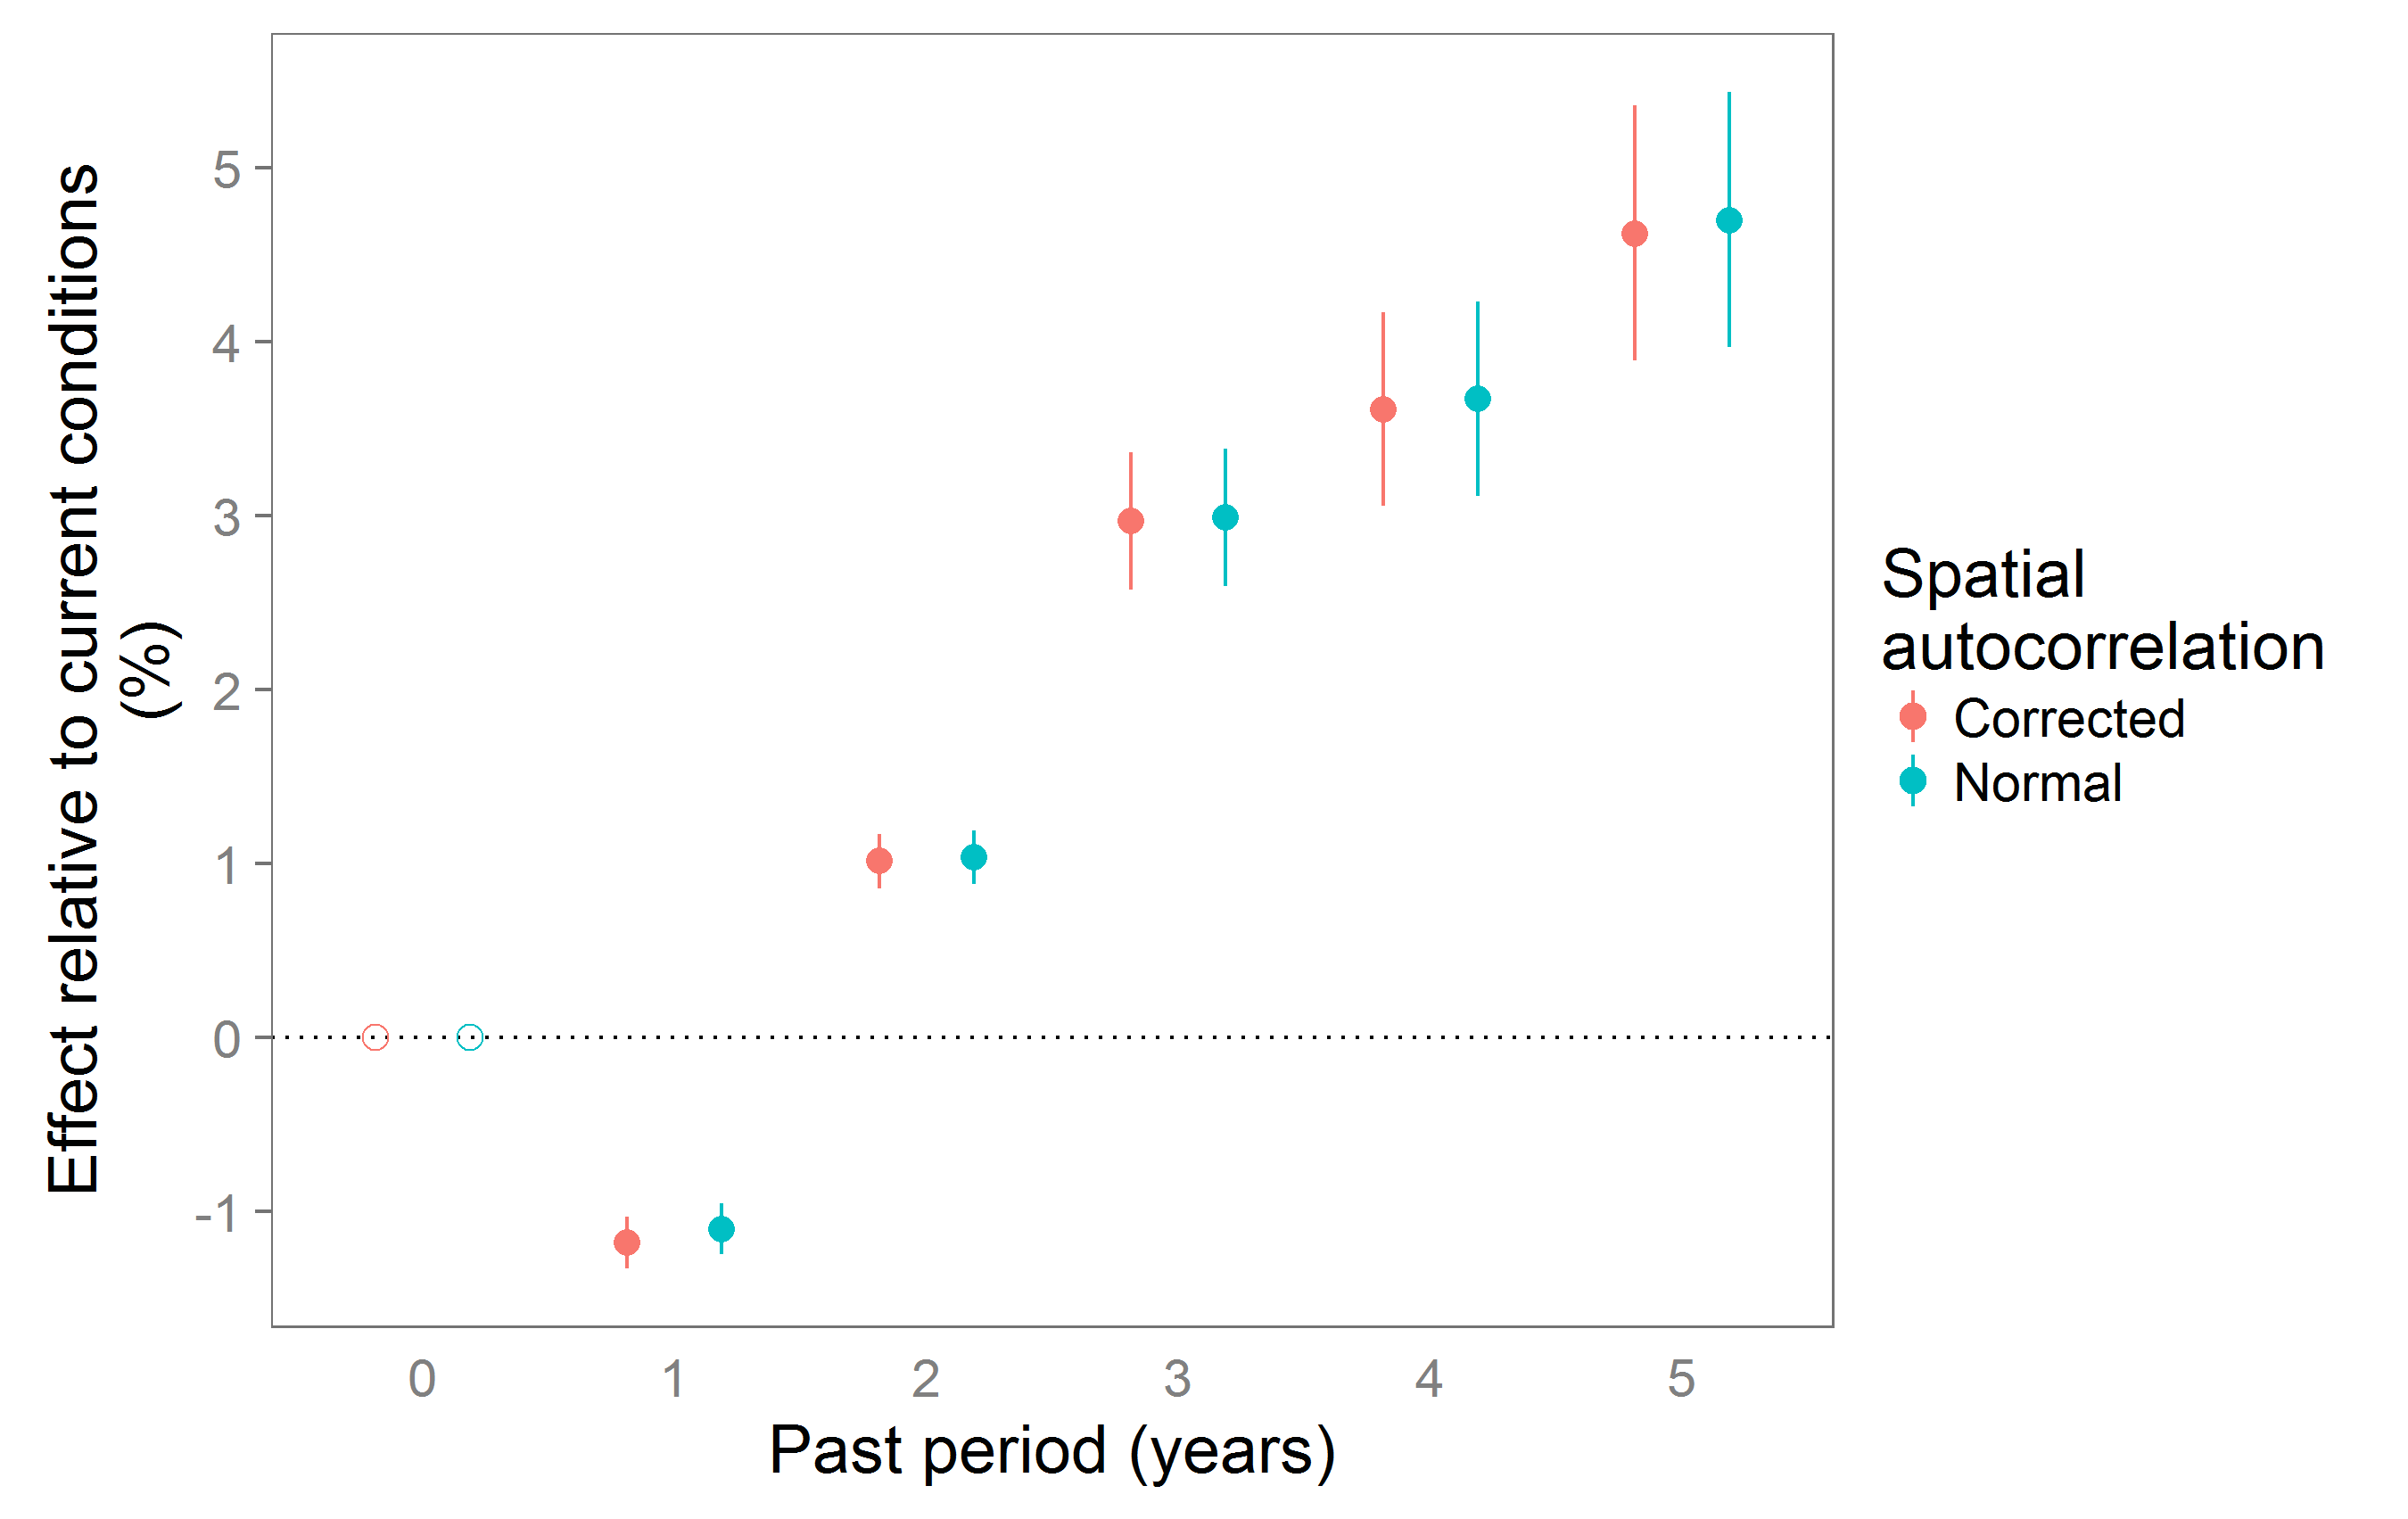
\includegraphics[width=1\textwidth]{chapter4/SI07}
\caption{As in Figure \ref{F04_05} but for species assemblage evenness (PIE). }
\label{SI04_07}
\end{figure}
